\usetikzlibrary{angles, quotes, calc}




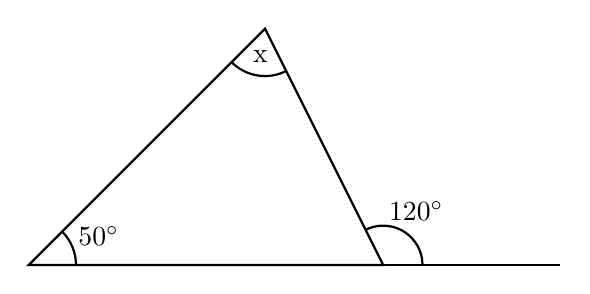
\begin{tikzpicture}[scale=1.5, line width=0.8pt]

    % --- Coordinates ---
    % Define points based on the geometry:
    % Exterior angle is 120, Interior angle at right is 180-120 = 60
    % Left angle is 50
    % Top angle x is 180 - (50+60) = 70
    
    \coordinate (A) at (0,0);       % Bottom-left vertex
    \coordinate (B) at (3,0);       % Bottom-right vertex
    \coordinate (C) at (2, 2);    % Top vertex (approximate position)
    
    % Recalculate C to be geometrically accurate for angles 50 and 60
    % Using intersections of lines
    
    
    \coordinate (D) at (4.5, 0);    % Extension point to the right

    % --- Draw Lines ---
    \draw (A) -- (B) -- (C) -- cycle; % The triangle
    \draw (B) -- (D);                 % The base extension

    % --- Draw Arcs & Labels ---

    % 1. Left Angle (50 degrees)
    % pic text options: shift moves label further out/in
    \draw pic["$50^{\circ}$", draw, angle radius=0.6cm, angle eccentricity=1.6] 
        {angle = B--A--C};

    % 2. Top Angle (x)
    % "x" is placed slightly lower than the arc center
    \draw pic["x", draw, angle radius=0.6cm, angle eccentricity=0.6] 
        {angle = A--C--B};

    % 3. Exterior Angle (120 degrees)
    % Note: angle is defined D-B-C
    \draw pic["$120^{\circ}$", draw, angle radius=0.5cm, angle eccentricity=1.6] 
        {angle = D--B--C};

\end{tikzpicture}